
\documentclass{article}
\usepackage{graphicx}
\usepackage[margin=1in]{geometry}
\title{Stock Report: AAPL}
\author{Jack Massey}
\date{\today}

\begin{document}
\maketitle

\section*{Summary}
\textbf{Period:} 2024-04-25 to 2025-04-24

\begin{itemize}
    \item Latest Close Price: 208.37 USD
    \item Growth (1Y): 23.23\%
    \item Volatility: 0.0207
    \item P/E Ratio: 33.13
    \item Market Cap: 3.13 Trillion
\end{itemize}

\section*{Today's Data}
\begin{tabular}{lr}\textbf{Metric} & \textbf{Value} \\
\hline
Open & 204.89 \\
High & 208.83 \\
Low & 202.94 \\
Close & 208.37 \\
Volume & 47,199,300.00 \\
Dividends & 0.00 \\
Stock Splits & 0.00 \\
Daily Return & 0.02 \\
50MA & 219.52 \\
200MA & 227.40 \\
EMA12 & 200.96 \\
EMA26 & 205.86 \\
MACD & -4.90 \\
Signal & -6.98 \\
Histogram & 2.09 \\
RSI & 52.40 \\
20MA & 202.28 \\
20STD & 14.36 \\
Upper Band & 231.01 \\
Lower Band & 173.55 \\
H-L & 5.89 \\
H-PC & 4.23 \\
L-PC & 1.66 \\
TR & 5.89 \\
ATR & 12.65 \\
OBV & 1,676,464,000.00 \\
%K & 89.55 \\
%D & 75.01 \\
\end{tabular}

\section*{Bollinger Bands}
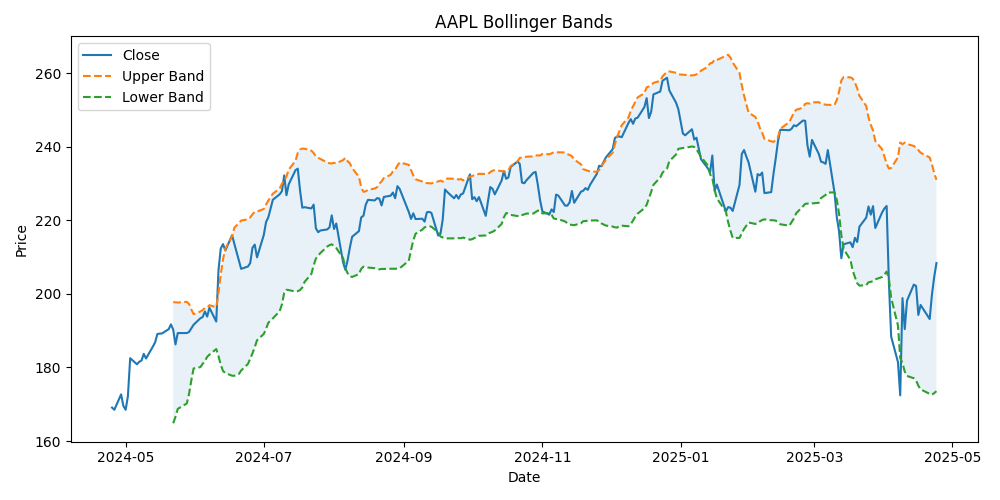
\includegraphics[width=\textwidth]{bollinger_AAPL_2025-04-25_10-43-40.png}

\textit{Close is between upper and lower bands, possibly indicating consolidation or pending breakout.}

\section*{MACD}
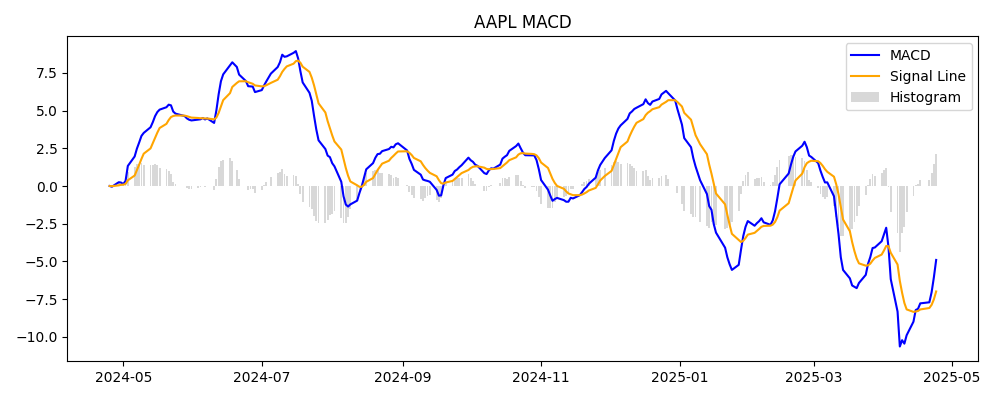
\includegraphics[width=\textwidth]{macd_AAPL_2025-04-25_10-43-40.png}

\textit{Look for signal line crossovers to identify bullish or bearish shifts in momentum.}

\section*{RSI}
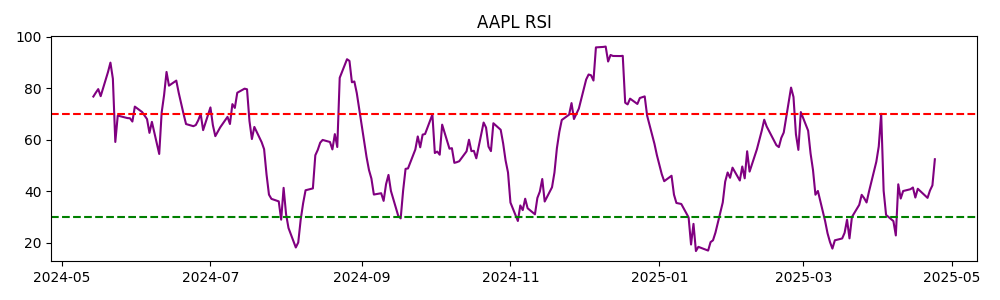
\includegraphics[width=\textwidth]{rsi_AAPL_2025-04-25_10-43-40.png}

\textit{RSI near 70 indicates overbought; near 30 suggests oversold.}

\section*{Insights}
AAPL shows recent volatility trends with Bollinger Bands and momentum signals through MACD and RSI. Review context in relation to market news or events.

\end{document}
